% !TEX root = ./main.tex
\graphicspath{{figures_cylinder/}}% Set graphics path location

\subsection{Circular Cylinder}

The classic test case of laminar flow past a circular cylinder at low Reynolds number has also been chosen as a verification and validation case for the 2D Navier-Stokes equations in HiFiLES, and the results are compared to existing experimental data and simulation results~\cite{park1998}. Two separate cases are computed: first, the steady flow past the cylinder at $Re = 20$, and second, the unsteady flow past the cylinder at $Re = 100$, where the Reynolds number is based upon the diameter of the cylinder. For both cases, the Mach number is set to 0.1 in order to recover nearly incompressible flow for comparisons with the existing incompressible results. The remaining flow conditions are 0$\degr$ angle of attack, a constant ratio of specific heats of $1.4$, a Prandtl number of $0.72$, a free-stream temperature of 300 $K$, and a free-stream dynamic viscosity of $1.853\cdot 10^{-5} Pa \cdot s$ (laminar viscosity varies according to Sutherland's law during the simulation).

The two simulations are performed with third order polynomials on a mesh with 4988 total elements that contains quadrilateral elements near the body of the cylinder and triangular elements out to the far-field. There is a small refinement box immediately downstream of the cylinder to help resolve features in the wake. The rectangular far-field boundaries are located approximately 30 diameters away from the cylinder in the upstream, upward, and downward directions and 50 diameters away in the downstream direction. A view of the mesh near the cylinder surface is shown in Fig.~\ref{cylinder_1}.

\begin{figure}
  \begin{subfigmatrix}{2}
    \subfigure[Zoom view of the mesh near the cylinder.]{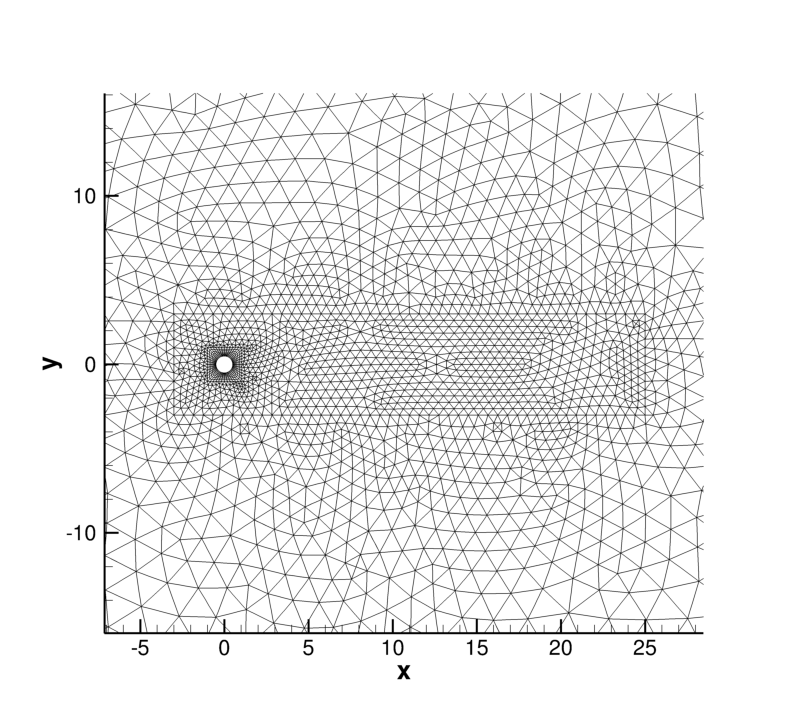
\includegraphics{cylinder_mesh.png}}
    \subfigure[X-velocity contours and streamlines around the circular cylinder for $Re = 20$.]{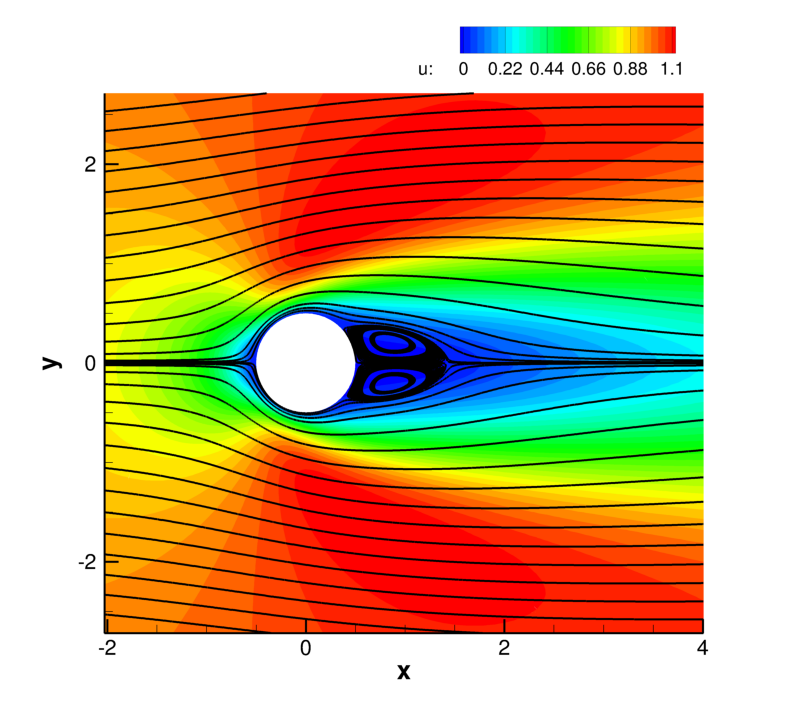
\includegraphics{cylinder_streamlines.png}}
  \end{subfigmatrix}
  \caption{The mesh for the circular cylinder simulations along with x-velocity contours for the $Re = 20$ case.}
  \label{cylinder_1}
\end{figure}

The flow around the cylinder for $Re = 20$ is steady, and it features a large recirculation region behind the cylinder. Fig.~\ref{cylinder_1} presents x-velocity contours around the cylinder along with streamlines. The length of the recirculation region can be determined from the streamlines, and a length of approximately one cylinder diameter agrees well with reported results for $Re = 20$. The coefficient of drag computed by HiFiLES is 2.043, which is close to the value of 2.01 reported by Park et al. Pressure contours around the cylinder are shown in Fig.~\ref{cylinder_2}.

\begin{figure}
  \begin{subfigmatrix}{2}
    \subfigure[Pressure contours for the $Re = 20$ case.]{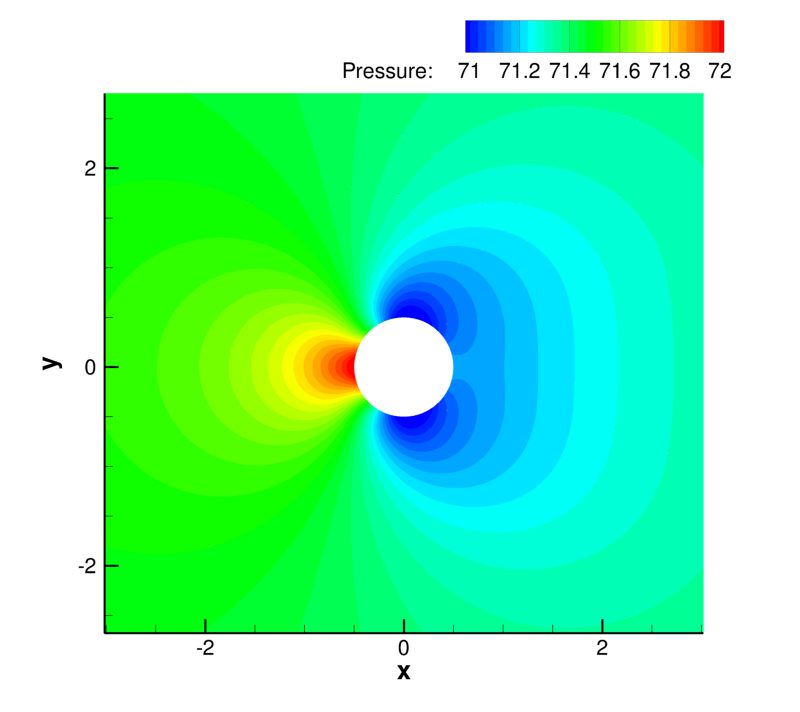
\includegraphics{cylinder_pressure_re20.png}}
    \subfigure[Pressure contours for the $Re = 100$ case.]{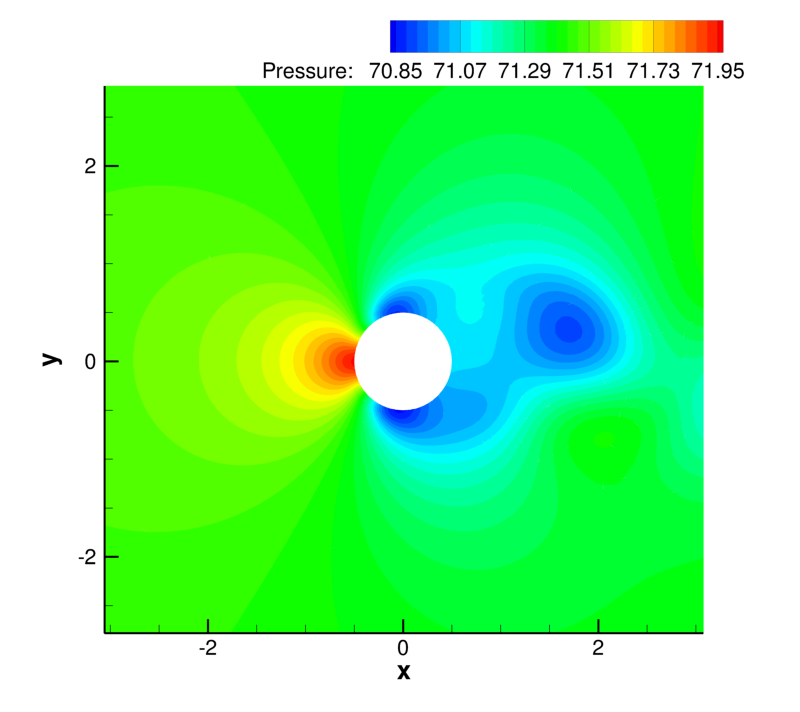
\includegraphics{cylinder_pressure_re100.png}}
  \end{subfigmatrix}
  \caption{Pressure contours for the steady and unsteady (instantaneous) cylinder cases.}
  \label{cylinder_2}
\end{figure}

When the Reynolds number is increased to 100, the flow around the cylinder becomes unsteady and exhibits periodic vortex shedding. This periodic shedding in the wake behind the cylinder can be seen in the instantaneous contours of x-velocity and vorticity in Fig.~\ref{cylinder_3}, and it also results in periodic fluctuations in the force coefficients on the cylinder. HiFiLES reports an average drag coefficient of 1.339 with a maximum deviation from this value of 0.0092, which agree excellently with the values reported by Park et al. of 1.33 and 0.0091 for the average $C_d$ and maximum deviation from it, respectively.  Instantaneous pressure contours for the $Re = 100$ case can be seen in Fig.~\ref{cylinder_2}. The asymmetry that is visible in the pressure contours contributes to the variability in the drag coefficient.

\begin{figure}
  \begin{subfigmatrix}{2}
    \subfigure[X-velocity contours around the circular cylinder for $Re = 100$.]{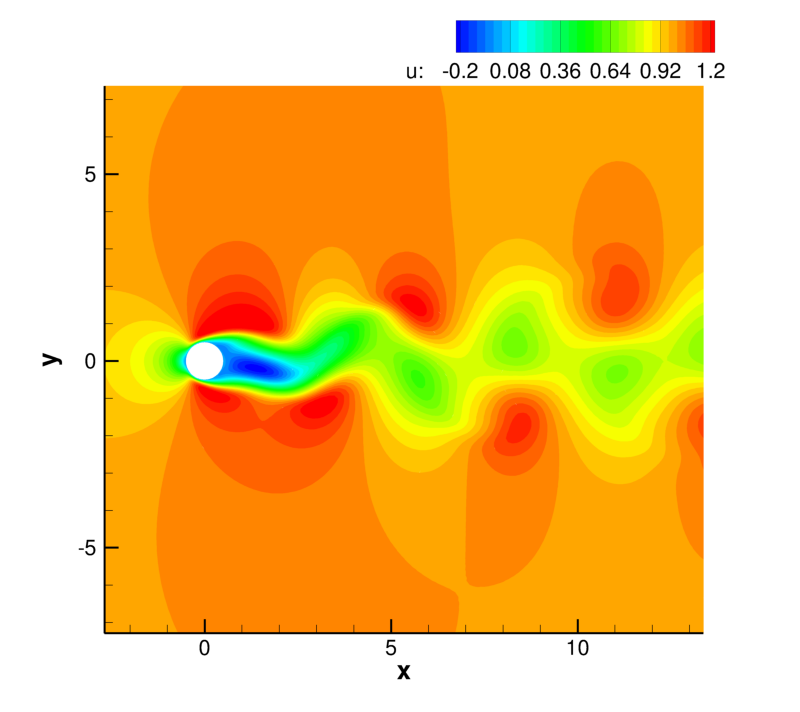
\includegraphics{cylinder_xvelocity_re100.png}}
    \subfigure[Vorticity contours for the $Re = 100$ case.]{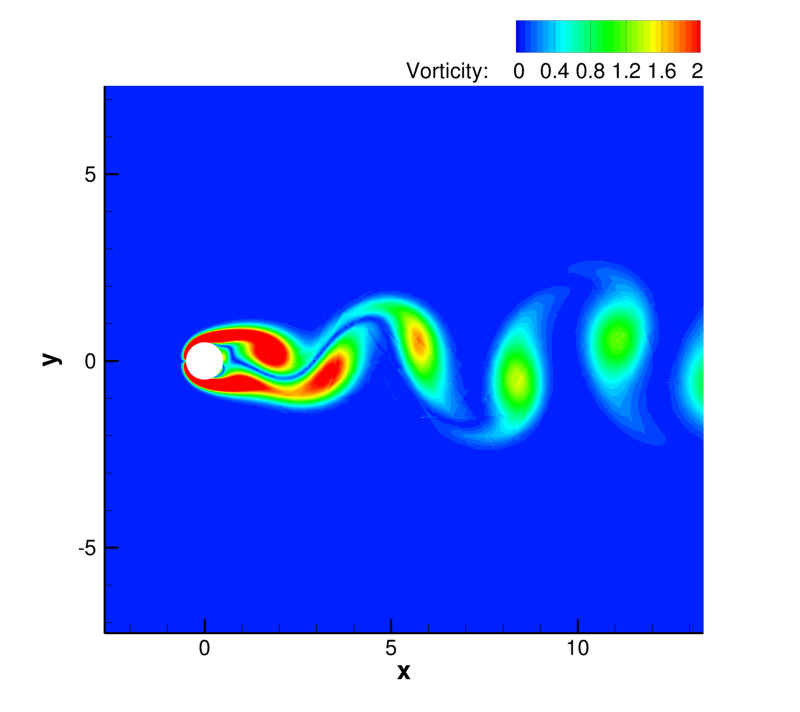
\includegraphics{cylinder_vorticity_re100.png}}
  \end{subfigmatrix}
  \caption{Instantaneous solution contours for the unsteady cylinder case.}
  \label{cylinder_3}
\end{figure}